\documentclass{article}

% Language setting
% Replace `english' with e.g. `spanish' to change the document language
\usepackage[english]{babel}

% Set page size and margins
% Replace `letterpaper' with `a4paper' for UK/EU standard size
\usepackage[letterpaper,top=2cm,bottom=2cm,left=3cm,right=3cm,marginparwidth=1.75cm]{geometry}

% Useful packages
\usepackage{amsmath}
\usepackage{amsfonts}
\usepackage{graphicx}
\usepackage[colorlinks=true, allcolors=blue]{hyperref}

\usepackage{natbib}

\title{Evolutionary Pair HMM}
\author{Ian Holmes}

\begin{document}
%\maketitle

\section{Statistical alignment}

\subsection{General geometric indel model (GGI)}

A sequence $S(t)$ evolves by
substitutions (rate matrix $Q$),
deletions (rate $\mu$ per site, extension probability $y$),
and
insertions (rate $\lambda$, extension $x$,
characters $\sim Q$'s stationary distribution $\pi$).

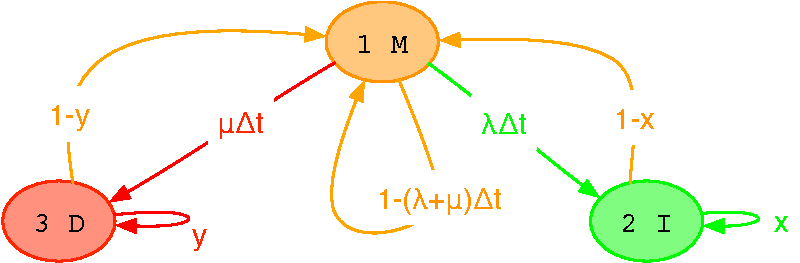
\includegraphics[width=\textwidth]{InstantHMM.pdf}

At equilibrium, sequence length $\sim$ Geometric($\lambda/\mu$). Composition is $\pi$.

If the model is required to be reversible then $\lambda y(1-x) = \mu x(1-y)$.

\subsection{Conditional Pair HMM (transducer) with time-dependent parameters}
Derived in \cite{Holmes2020}.
A Pair HMM whose state path likelihood approximates $P(S(t)|S(0))$

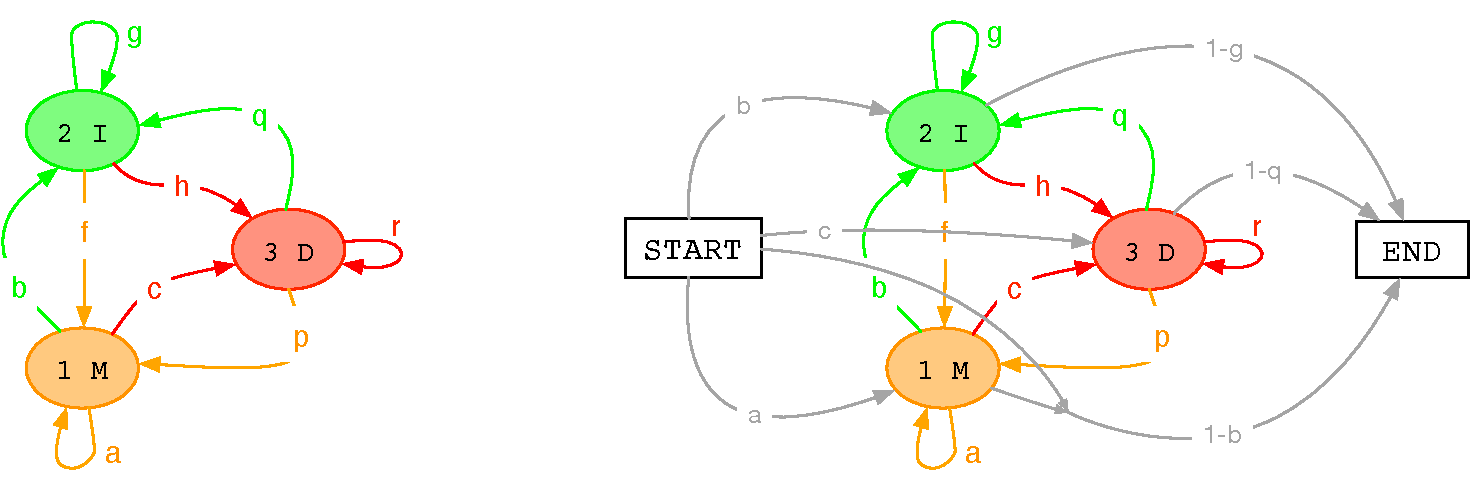
\includegraphics[width=\textwidth]{PairHMM.pdf}

At $t=0$: $a(0)=1$, $f(0)=1-x$, $g(0)=x$, $p(0)=1-y$, $r(0)=y$, and $b(0)=c(0)=h(0)=q(0)=0$.

For $t>0$, % following Holmes (2020)
\begin{eqnarray*}
\begin{bmatrix}
a & b & c \\
f & g & h \\
p & q & r 
\end{bmatrix}
& = &
\begin{bmatrix}
T_{MM} & T_{MI} & 1-T_{MM}-T_{MI} \\
T_{IM}/W_I & (W_I-T_{MI}-T_{DI})/W_I & (T_{MI}+T_{DI}-T_{IM})/W_I \\
(1-T_{MM}-T_{IM})/W_D & T_{DI}/W_D & (W_D+T_{MM}+T_{IM}-T_{DI}-1)/W_D 
\end{bmatrix}
\\
W_I(t) & = & \exp\left(\frac{\lambda t}{1-x}\right)-1 \\
W_D(t) & = & \exp\left(\frac{\mu t}{1-y}\right)-1 \\
T_{ij}(0) & = & \mbox{1 if $i=j=M$, 0 otherwise}
\\
  \frac{d}{dt} T_{MM}(t) & = &
  \mu \frac{b f (1-y)}{1 - g y}-(\lambda +\mu )a
  \nonumber \\
  \frac{d}{dt} T_{MI}(t) & = &
  -\mu \frac{b (1-g)}{1 - g y} + \lambda (1-b)
  \nonumber \\
  \frac{d}{dt} T_{IM}(t) & = &
  \lambda a - \mu \frac{f (1-g) (b (1-r)+c q)}{(1 - g y) (f (1-r)+h p)}
  \nonumber \\
  \frac{d}{dt} T_{DI}(t) & = &
  \mu \frac{(1-g) (b (1-r-h q)+c g q)}{(1-g y) (f (1-r)+h p)}
\end{eqnarray*}

The $T_{ij}(t)$ may be approximated by Runge-Kutta methods,
e.g. Dormand-Prince. % \cite{DormandPrince1980}

The substitution matrix for the M state of the Pair HMM is
the matrix exponential $\exp(Qt)$, for which a Pad\'{e} approximant
or other power series expansion can be used. % \cite{MolerVanLoan2003}

\subsection{Exactly-solved special case (TKF91)}

When $x=y=0$ the model is TKF91 \cite{ThorneEtAl91}
with solution
$
\begin{bmatrix}
a & b & c \\
f & g & h \\
p & q & r 
\end{bmatrix}
=
\begin{bmatrix}
(1-\beta)\alpha & \beta & (1-\beta)(1-\alpha) \\
(1-\beta)\alpha & \beta & (1-\beta)(1-\alpha) \\
(1-\gamma)\alpha & \gamma & (1-\gamma)(1-\alpha)
\end{bmatrix}
$
where
$\alpha = \exp(-\mu t)$,
$\beta = \frac{\lambda \left( \exp(-\lambda t) - \exp(-\mu t) \right)}{\mu \exp(-\lambda t) - \lambda \exp(-\mu t)}$
and
$\gamma = 1 - \frac{\mu \beta}{\lambda (1 - \alpha)}$.



\subsection{Alignment unspecified}

Suppose a prefix list (or tree) of sequences.
Node 1 corresponds to the empty sequence.
Nodes $N>1$ correspond to nonempty sequences $S_N$.
Character $\omega_N$ is the last character of $S_N$.
The parent node $\psi_N$ corresponds to the longest prefix of $S_N$:
removing $\omega_N$ from $S_N$ leaves $S_{\psi_N}$.

Let $F(i,j,t) = \begin{bmatrix} F_M & F_I & F_D \end{bmatrix}$
be the per-state Forward likelihoods for sequences $S_i,S_j$.

We seek $F^\dagger(i,j,t) = P(S(t)=S_j|S(0)=S_i)$.
The Forward recursions are, for $i>1$ and $j>1$
\begin{eqnarray*}
F(1,1,t) & = & \begin{bmatrix} 1 & 0 & 0 \end{bmatrix}
\\
F(1,j,t) & = &
F(1,\psi_j,t) U_I(\omega_j,t)
\\
F(i,1,t) & = &
F(\psi_i,1,t) U_D(\omega_i,t)
\\
F(i,j,t) & = &
F(\psi_i,\psi_j,t) U_M(\omega_i,\omega_j,t)
+ F(i,\psi_j,t) U_I(\omega_j,t)
+ F(\psi_i,j,t) U_D(\omega_i,t)
\\
F^\dagger(i,j,t) & = & F(i,j,t) \begin{bmatrix}
1-b(t) \\
1-g(t) \\
1-q(t) \end{bmatrix}
\\
U_M(\omega_i,\omega_j,t) & = &
\begin{bmatrix}
a(t) & 0 & 0 \\
f(t) & 0 & 0 \\
p(t) & 0 & 0 
\end{bmatrix}
\exp(Qt)_{\omega_i \omega_j}
\\
U_I(\omega_j,t) & = &
\begin{bmatrix}
0 & b(t) & 0 \\
0 & g(t) & 0 \\
0 & q(t) & 0 
\end{bmatrix}
\pi_{\omega_j}
\\
U_D(\omega_i,t) & = &
\begin{bmatrix}
0 & 0 & c(t) \\
0 & 0 & h(t) \\
0 & 0 & r(t) 
\end{bmatrix}
\end{eqnarray*}

The time complexity to compute the Forward likelihood is $O(L^2)$,
where $L$ is the sequence length.

\subsection{Alignment specified}

The pairwise alignment of ancestor $i$ and descendant $j$ can be summarized by two lists:
\begin{itemize}
    \item The list $A_M$ of pairs of aligned characters $(\omega,\omega')$ from ancestor $S(0)$ and descendant $S(t)$;
    \item The list $A_{ID}$ of pairs of unaligned gap sequences $(\delta,\delta')$ that were deleted and inserted in between.
\end{itemize}

The alignment probability, computable in time $O(L)$ (and in practice very fast), is
\[
P(A_M,A_{ID},S(t)|S(0)) =
\prod_{(\omega,\omega') \in A_M} \exp(Qt)_{\omega \omega'}
\prod_{(\delta,\delta') \in A_{ID}} G(|\delta|,|\delta'|,t)
\prod_{\omega'\in \delta'} \pi_{\omega'}
\]

where $G(i,j,t)$ is the probability that between the next pair of aligned characters in $S(0)$ and $S(t)$,
there were $i$ characters deleted from $S(0)$ 
and $j$ characters inserted into $S(t)$,
with no homology
\begin{eqnarray*}
G(0,0,t) & = & a \\
G(i,0,t) & = & cr^{i-1}p \\
G(0,j,t) & = & bg^{j-1}f \\
G(i,j,t) & = &
g^{j-1} r^{i-1}
\sum_{k=0}^{\min(i,j)}
\left(\frac{hq}{gr}\right)^k
\left[
\binom{i}{k} \binom{j-1}{k} brf
+ \binom{i-1}{k} \binom{j-1}{k} (bhp+cqf)
+ \binom{i-1}{k} \binom{j}{k} cgp
\right]
\end{eqnarray*}
% The unobserved index $k$ counts zig-zags on the Pair HMM state path
% ($D \to I \to D$ or $I \to D \to I$).

\subsection{Phylogenetic alignment}

Both forms of the pairwise likelihood (alignment specified, or unspecified) can be extended to multiple sequences on a phylogeny.
Upgrade $\exp(Qt)$ to Felsenstein pruning. % \cite{Felsenstein81}.

For the alignment-unspecified form, use automata composition to obtain $N$-sequence HMMs \cite{SilvestreRyanEtAl2020}.
The resulting Forward algorithm is $O(L^N)$.
This can be reduced to $O(L^2)$ by MCMC \cite{RedelingsSuchard2007}
and further improved by sampling \cite{WestessonEtAl2012}
and adaptive dynamic programming \cite{DeMaio2020}.

\section{Potts Hamiltonian}

Suppose that the $L$-character sequence
is selected from a Potts Hamiltonian
\begin{eqnarray*}
P(S) & = & \frac{1}{Z} \exp(H(S)) \\
H(S_1 \ldots S_L) & = &
\sum_{i=1}^L h_i(S_i)
+
\sum_{i=1}^L \sum_{i<j}^L J_{ij}(S_i,S_j)
\\
Z & = & \sum_S \exp(H(S))
\end{eqnarray*}


\section{Grammatically structured indel model (GSI)}

Consider a stochastic context-free grammar ${\cal G}$
with nonterminals ${\cal W}$ and terminals $\Omega$.

Let $\Upsilon$ be the set of parse trees for this grammar
and let $X,Y \in {\cal W}\cup\Omega$ denote grammar symbols.

We describe a continuous-time Markov chain (CTMC) with $\Upsilon$ as a state space.
By construction, ${\cal G}$ gives the equilibrium distribution over $\Upsilon$.
We also describe a pair grammar ${\cal G}_t$ that computes matrix exponentials of this CTMC's rate matrix.

\subsection{Rate matrix}

Let some subset of nonterminals be designated as {\em substitution states}.
All outgoing rules from these symbols must be of the form $W \to X$.
The rule expansion used in the parse tree evolves as a continuous-time Markov chain,
changing from $W \to X$ to $W \to Y$ with rate $Q^{(W)}_{XY}$.
Any recursive grammatical expansion of $X$ further down the parse tree
is resampled instantaneously whenever the rule expansion changes.
The stationary distribution $\pi^{(W)}_X$ of the rate matrix $Q^{(W)}$ is the rule probability $P(W \to X|G)$.

Let some other subset of nonterminals be designated as {\em link states}.
All outgoing rules from these symbols must be of the form $W \to X W$ or $W \to \epsilon$.
Such rules expand to become a sequence of $X$'s in the parse tree.
This sequence evolves over time as a self-contained geometric general indel model.
The parameters of this model are $(\lambda_W, \mu_W, x_W, y_W)$
where $\pi^{(W)}_X = P(W \to X|G) / (\lambda_W / \mu_W)$ is the distribution over elements in the list
and $\lambda_W / \mu_W = 1 - P(W \to \epsilon|G)$ is the geometric parameter of the list length distribution at equilibrium.
This GGI model does not itself have a substitution model built into it,
but the elements of the list can themselves be state variables;
for example, $X$ can itself be a substitution or link state,
or it can expand to a sequence of such symbols.

\subsection{Pair grammar}

We construct the pair grammar ${\cal G}_t$ whose Inside likelihood is the joint probability $P(S(0),S(t))$
by first creating copies ${\cal G}_1$ and ${\cal G}_2$ of the original grammar ${\cal G}$,
each copy having nonterminals $({\cal W}_1,{\cal W}_2)$ and terminals $(\Omega_1,\Omega_2)$ respectively.
(Suffix 1 denotes ancestor $S(0)$ and suffix 2 descendant $S(t)$.)

Next, we create a copy ${\cal G}_t$ of ${\cal G}$ with implicit rules $\omega_t \to \omega_1 \omega_2$.

In ${\cal G}_t$, the substitution rules $W \to X$ of ${\cal G}$ are replaced by rules

\[
\begin{array}{rclll}
  W_t & \to & X_t & & \pi^{(W)}_X \exp(Q^{(W)}_{XX} t) \\
      & | & X_1 & Y_2 & \pi^{(W)}_X (\exp(Q^{(W)} t)_{XY} - \delta_{XY} \exp(Q^{(W)}_{XX} t)) \\
\end{array}
\]

Also in ${\cal G}_t$, the link rules $W \to X W$ and $W\to\epsilon$ of ${\cal G}$ are replaced by rules

\[
\begin{array}{rclll}
  W_t & \to & X_t & W_t & (\lambda_W/\mu_W) a_W \pi^{(W)}_X  \\
      & | & X_2 & W_I & b_W \pi^{(W)}_X \\
      & | & X_1 & W_D & (\lambda_W/\mu_W) c_W \pi^{(W)}_X \\
      & | & \epsilon & & (1 - \lambda_W/\mu_W) (1-b_W) \\
  W_I & \to & X_t & W_t & (\lambda_W/\mu_W) f_W \pi^{(W)}_X \\
      & | & X_2 & W_I & g_W \pi^{(W)}_X \\
      & | & X_1 & W_D & (\lambda_W/\mu_W) h_W \pi^{(W)}_X \\
      & | & \epsilon & & (1 - \lambda_W/\mu_W) (1-g_W) \\
  W_D & \to & X_t & W_t & (\lambda_W/\mu_W) p_W \pi^{(W)}_X \\
      & | & X_2 & W_I & q_W \pi^{(W)}_X \\
      & | & X_1 & W_D & (\lambda_W/\mu_W) r_W \pi^{(W)}_X \\
      & | & \epsilon & & (1 - \lambda_W/\mu_W) (1-q_W) \\
\end{array}
\]

\section{Context-sensitive TKF91}

As long as we are introducing latent information...

In this version of TKF91, there is only insertion and deletion of links; no substitution.
There are $K$ types of mortal link.
At equilibrium, the probability of observing sequence $S$
is
\[
\Phi(S_1 \ldots S_L) =
\phi(\omega'=S_1|\omega=\epsilon)
\left( \prod_{i=1}^{L-1} \phi(\omega'=S_{i+1}|\omega=S_i) \right)
\phi(\omega'=\epsilon|\omega=S_L)
\]
where $\phi(\omega,\omega')$ is a joint distribution over adjacent link types,
with $\omega=\epsilon$ and $\omega'=\epsilon$ representing the ends of the sequence.

The insertion rate $\omega_i \omega_k \to \omega_i \omega_j \omega_k$
is $\lambda \phi(\omega_k|\omega_j) \phi(\omega_j|\omega_i)$.

The deletion rate $\omega_i \omega_j \omega_k \to \omega_i \omega_k$
is $\mu \phi(\omega_k|\omega_i)$.

Can we give this the renormalization treatment, e.g. by summarizing the path in terms of counts of adjacent types $(\omega,\omega')$?
Probably. But we don't need to. In the limit of very low indel rates, it's sufficient to consider 2-, 1-, or even 0-event trajectories.
The 0-event limit just gives you the phylo-HMM with transition matrix $\phi$.


\bibliographystyle{unsrt}
\bibliography{references}


\end{document}
